\documentclass{svproc}
\usepackage{url}
\usepackage{graphicx}
\def\UrlFont{\rmfamily}

\begin{document}
\mainmatter

\title{RSP-ViT: A Lightweight Shared-Parameter Vision Transformer for Human Activity Recognition from FMCW Radar Micro-Doppler Signatures}
\titlerunning{RSP-ViT for Radar Micro-Doppler Recognition}
\author{First Author \and Second Author}
\authorrunning{First Author et al.}
\institute{Affiliation}
\maketitle

\begin{abstract}
Human activity recognition based on radar micro-Doppler signatures has attracted increasing attention for privacy-preserving and contactless sensing. This paper presents a complete framework for FMCW radar-based activity recognition, including micro-Doppler image generation and lightweight classification. A practical 2D FFT-based signal processing pipeline is adopted to transform raw radar echoes into recognition-oriented micro-Doppler representations. On this basis, a lightweight recognition model termed RSP-ViT is proposed by combining a ResNet-style convolutional stem with shared-parameter transformer encoding. Experimental results show that the proposed method achieves a favorable trade-off between recognition accuracy and model efficiency when compared with a vanilla vision transformer and representative lightweight baselines.
\keywords{FMCW radar, micro-Doppler, human activity recognition, vision transformer, lightweight model}
\end{abstract}

\section{Introduction}

Radar-based human activity recognition has become an important research topic for privacy-preserving and contactless perception in healthcare, smart-home, and security applications \cite{Vandersmissen2018}. Compared with camera-based sensing, radar systems are less sensitive to illumination variation, partial occlusion, and adverse weather conditions, which makes them attractive for practical deployment. In an FMCW radar system, body-part motions such as arm swings, leg movements, and torso displacement induce characteristic micro-Doppler modulations that reveal fine-grained human motion dynamics \cite{Chen2006}. These motion patterns are commonly transformed into time-frequency representations to support subsequent recognition \cite{Harmanny2014}.

Early learning-based studies demonstrated that deep networks can identify human gait and activity patterns from radar micro-Doppler measurements with promising accuracy \cite{Papanastasiou2021}. Subsequent work extended radar-based recognition toward more general activity analysis and improved learning under limited labeled data \cite{Li2022SemiHAR}. Sequence-aware architectures further showed that explicit temporal modeling is beneficial when radar signatures evolve continuously over time \cite{Du2020SCGRNN}. More recently, hybrid transformer-based designs have been explored for radar human activity recognition, indicating the potential of combining convolutional priors with global dependency modeling \cite{Huan2023LHViT}.

From a model-design perspective, residual convolutional networks remain effective for stable optimization and local pattern extraction \cite{He2016ResNet}. MobileNetV2 provides a representative lightweight baseline for efficient deployment \cite{Sandler2018MobileNetV2}. In contrast, the Vision Transformer offers stronger long-range modeling capability through self-attention \cite{Dosovitskiy2021ViT}. However, when directly applied to micro-Doppler images, a vanilla vision transformer still suffers from weak local inductive bias and non-negligible parameter redundancy, which limits its suitability for lightweight radar perception tasks.

To address these issues, this paper proposes a lightweight recognition model termed RSP-ViT, short for ResNet-Stem Shared-Parameter Vision Transformer. The proposed architecture introduces a ResNet-style convolutional stem before token embedding to strengthen local feature extraction, while parameter sharing is employed across transformer layers to reduce model complexity. In addition, a practical 2D FFT-based signal processing pipeline is adopted to convert raw FMCW radar echoes into micro-Doppler images, thereby establishing a complete framework from radar signal acquisition to activity classification.

The contributions of this work are summarized as follows. First, a practical 2D FFT-based micro-Doppler image generation pipeline is established for FMCW radar data, which explicitly links raw radar echoes to recognition-oriented time-frequency representations. Second, a lightweight recognition model, termed RSP-ViT, is developed by combining a ResNet-style convolutional stem with shared-parameter transformer encoding to improve the accuracy-efficiency trade-off for micro-Doppler recognition. Third, extensive experiments are conducted against a vanilla vision transformer and representative lightweight baselines, showing that the proposed model outperforms the original transformer baseline and achieves a favorable balance between recognition accuracy and model efficiency.

\section{Radar Signal Processing and Micro-Doppler Generation}

To establish a complete sensing-to-recognition framework, the input images used in this work are generated from raw FMCW radar echoes through a standard 2D FFT-based preprocessing pipeline. The purpose of this stage is to convert complex radar measurements into a compact time-frequency representation that preserves motion-dependent characteristics for subsequent activity recognition. The overall processing flow adopted in this study is illustrated in Fig.~\ref{fig:pipeline_overview}.

\begin{figure}[t]
\centering
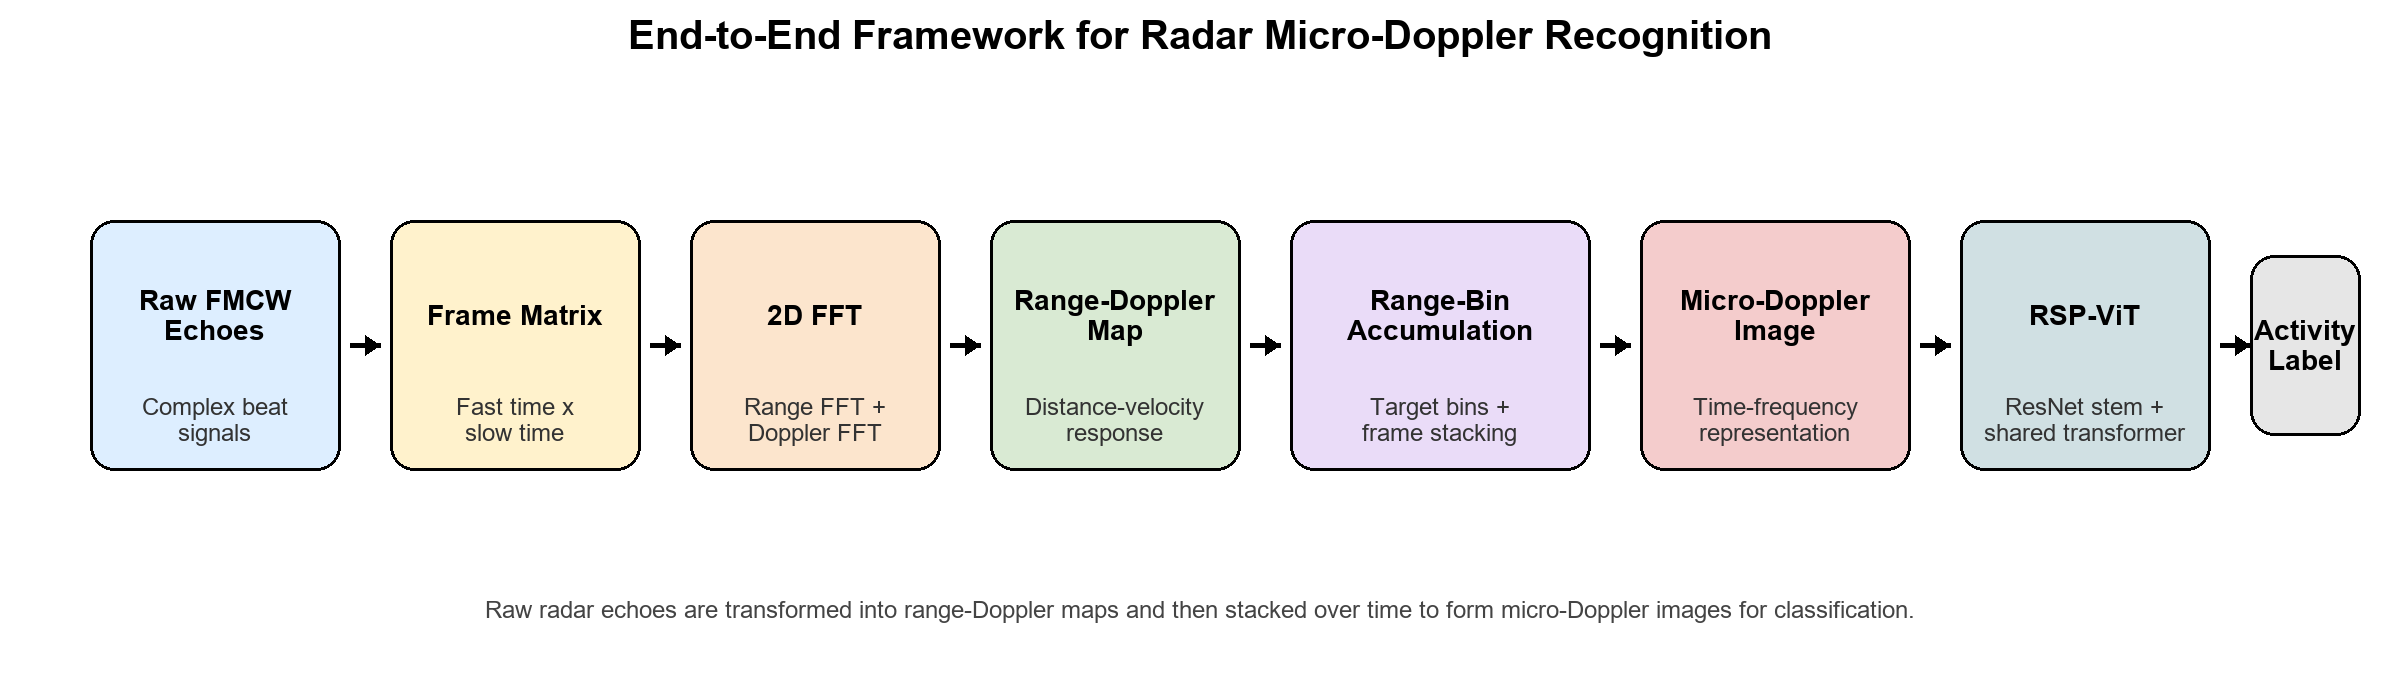
\includegraphics[width=0.98\textwidth]{figures/pipeline_overview.png}
\caption{Overall processing flow from raw FMCW radar echoes to activity recognition.}
\label{fig:pipeline_overview}
\end{figure}

\subsection{FMCW Radar Configuration}

The main radar parameters used for data acquisition are listed in Table~\ref{tab:radar_parameters}. The system operates at 77~GHz with a bandwidth of 768~MHz. For each pulse, 256 sampling points are collected at an ADC sampling frequency of 6~MHz. Each frame contains 255 pulses, and 1000 frames are recorded with a frame period of 13~ms. These settings provide sufficient temporal continuity and frequency resolution for capturing fine-grained human motion signatures.

\begin{table}[t]
\caption{Radar parameter configuration.}
\label{tab:radar_parameters}
\centering
\begin{tabular}{ll}
\hline
Parameter name & Set value \\
\hline
Carrier frequency & 77~GHz \\
Bandwidth & 768~MHz \\
ADC sampling frequency & 6~MHz \\
Number of sampling points per pulse & 256 \\
Number of pulses per frame & 255 \\
Number of frames & 1000 \\
Frame period & 13~ms \\
\hline
\end{tabular}
\end{table}

\subsection{2D FFT-Based Range-Doppler Processing}

For each frame, the sampled beat signals are arranged into a two-dimensional matrix, where the fast-time dimension corresponds to samples within a pulse and the slow-time dimension corresponds to pulses within a frame. A range FFT is first performed along the fast-time dimension to separate reflections at different distances. A Doppler FFT is then applied along the slow-time dimension to estimate velocity-related frequency shifts, thereby generating a range-Doppler map for each frame \cite{Chen2006}. In this way, the two-dimensional transform provides a joint description of target distance and radial motion.

\subsection{Micro-Doppler Image Generation}

The range-Doppler map of a single frame reflects the instantaneous energy distribution in the range-velocity plane. To characterize human motion over time, the Doppler responses associated with target-related range bins are accumulated for each frame and then stacked across consecutive frames. The resulting micro-Doppler image uses slow time as the horizontal axis, Doppler frequency or radial velocity as the vertical axis, and echo intensity as the pixel value \cite{Harmanny2014}. Since different activities produce different temporal Doppler evolution patterns, this representation is well suited for image-based human activity recognition. In this work, the generated micro-Doppler images are used as the input to the proposed RSP-ViT model. Representative examples from the dataset are shown in Fig.~\ref{fig:microdoppler_examples}.

\begin{figure}[t]
\centering
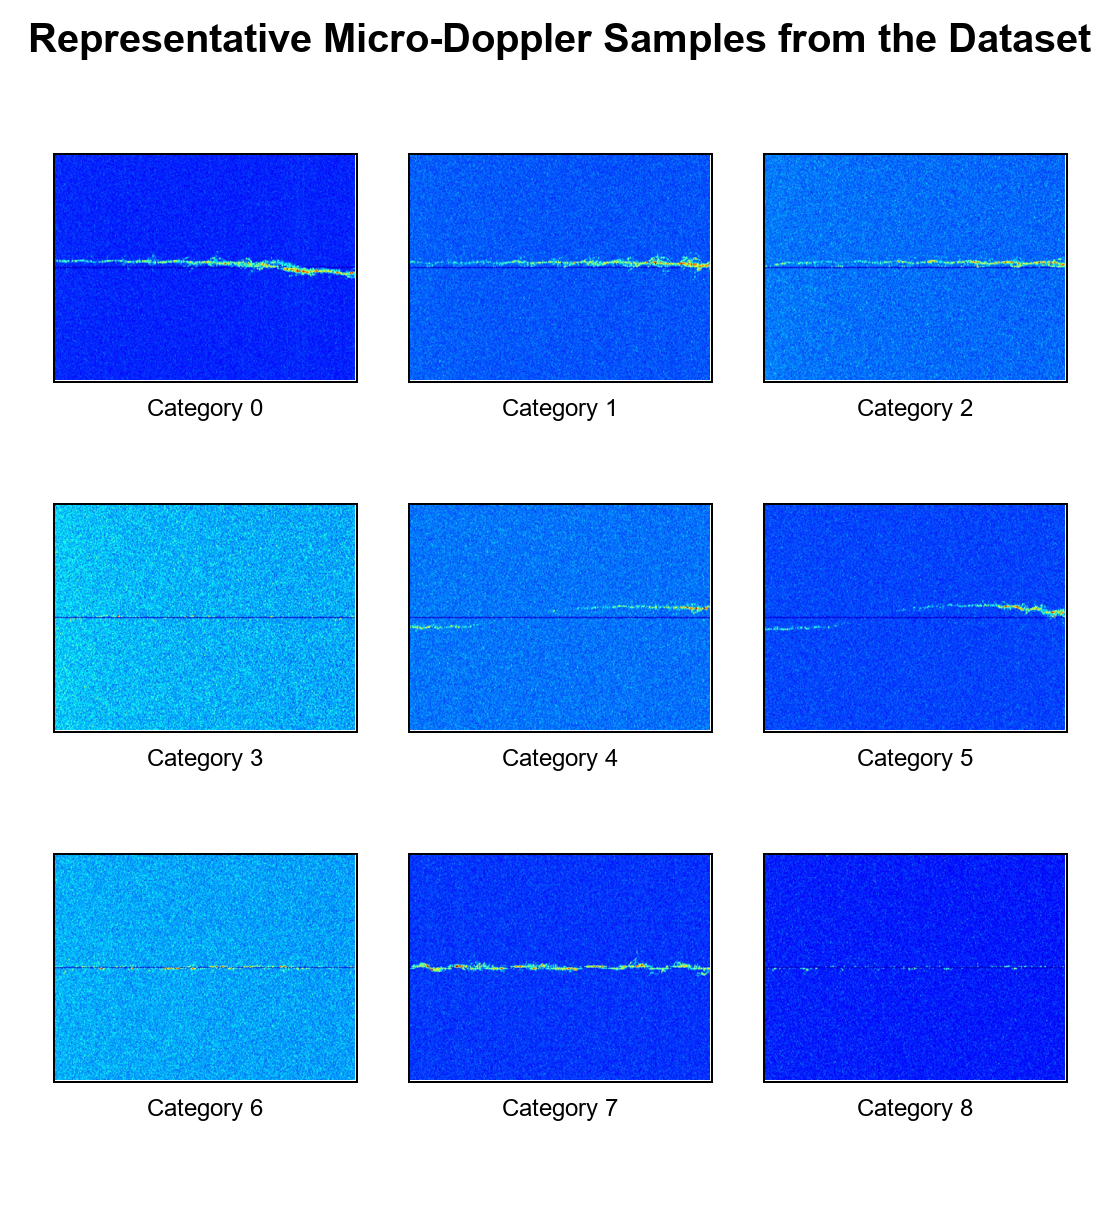
\includegraphics[width=0.92\textwidth]{figures/microdoppler_examples.png}
\caption{Representative micro-Doppler samples from the nine activity categories. The numeric labels correspond to the dataset category indices.}
\label{fig:microdoppler_examples}
\end{figure}

\section{Proposed RSP-ViT Model}

This section presents the proposed RSP-ViT, short for ResNet-Stem Shared-Parameter Vision Transformer. The model is designed for micro-Doppler image recognition, where both local texture continuity and global dependency modeling are important. As shown in Fig.~\ref{fig:rspvit_framework}, the proposed architecture contains three main components: a lightweight convolutional stem for local feature extraction, a transformer encoder with shared parameters for global representation learning, and a classification head for activity prediction.

\begin{figure}[t]
\centering
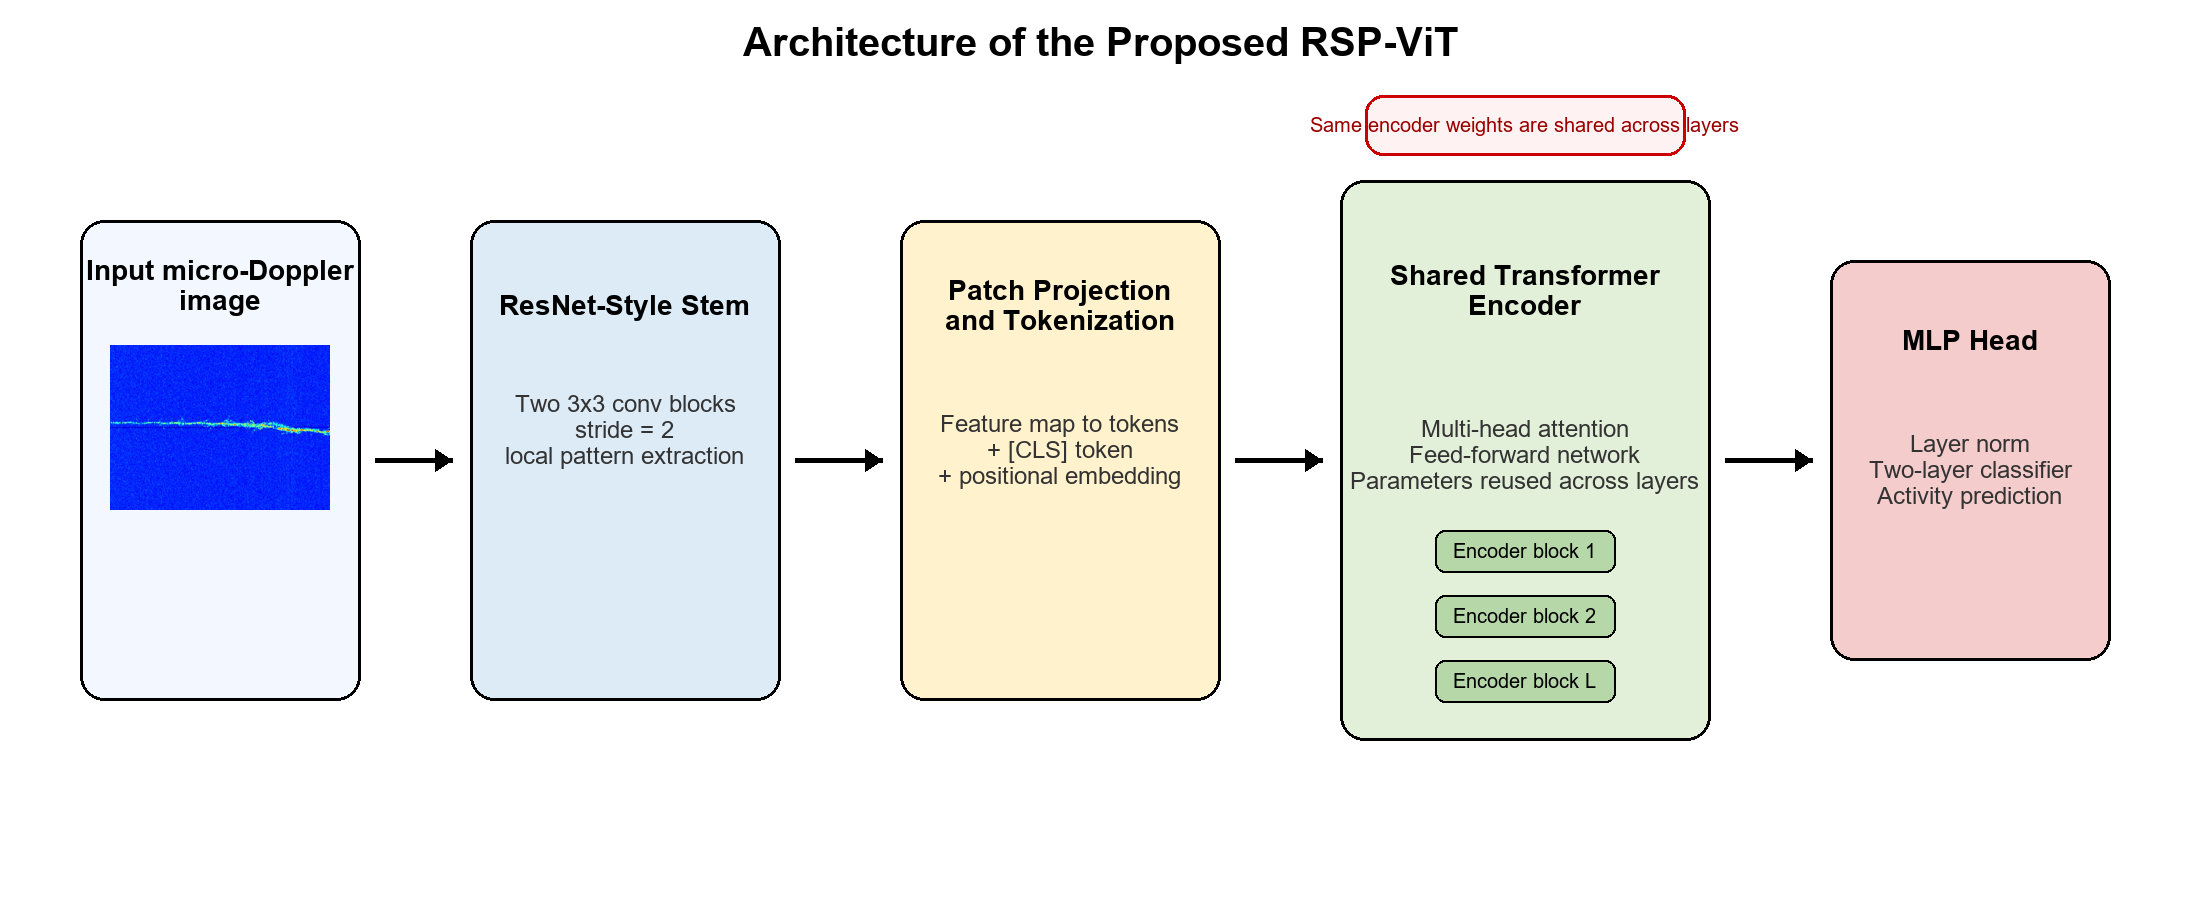
\includegraphics[width=0.98\textwidth]{figures/rspvit_architecture.png}
\caption{Overall architecture of the proposed RSP-ViT model.}
\label{fig:rspvit_framework}
\end{figure}

\subsection{Overall Architecture}

Let the input micro-Doppler image be denoted by $I$. The image is first processed by a convolutional stem to enhance local motion patterns before tokenization. The resulting feature map is then converted into a token sequence and combined with a learnable classification token and positional embeddings. After that, the token sequence is fed into $L$ transformer encoder layers. Finally, the output feature corresponding to the classification token is passed to a two-layer multilayer perceptron for category prediction. The overall forward process can be written as
\begin{equation}
Z_0 = \mathrm{Tokenize}(\mathrm{Stem}(I)) + E_{\mathrm{pos}},
\end{equation}
\begin{equation}
Z_l = \mathcal{T}_{\theta}(Z_{l-1}), \quad l=1,2,\ldots,L,
\end{equation}
\begin{equation}
\hat{y} = \mathrm{Head}(Z_L^{\mathrm{cls}}),
\end{equation}
where $\mathcal{T}_{\theta}(\cdot)$ denotes the shared transformer encoder, $E_{\mathrm{pos}}$ denotes positional embeddings, and $Z_L^{\mathrm{cls}}$ denotes the final classification token.

\subsection{ResNet-Style Convolutional Stem}

In a vanilla vision transformer, image patches are directly projected into token embeddings by a single patchifying operation \cite{Dosovitskiy2021ViT}. However, micro-Doppler images contain fine local structures, such as narrow Doppler ridges, periodic streaks, and short-term texture transitions, which are more effectively captured by convolutional operations. Therefore, RSP-ViT introduces a lightweight ResNet-style stem before token embedding. Specifically, two successive $3 \times 3$ convolutional blocks with stride 2 are used to progressively extract local patterns and reduce the spatial resolution. A patch projection layer is then applied to map the convolutional features into transformer tokens. This design strengthens local inductive bias while keeping the subsequent transformer interface unchanged. It is also consistent with the effectiveness of residual-style convolutional feature extraction in visual recognition tasks \cite{He2016ResNet}.

\subsection{Shared-Parameter Transformer Encoder}

After tokenization, the feature sequence is modeled by a stack of transformer encoder layers. Each encoder layer contains multi-head self-attention and a feed-forward network with residual connections and layer normalization. Different from a standard vision transformer, RSP-ViT adopts layer-wise parameter sharing, that is, the same encoder parameters are reused across multiple transformer depths. This strategy is inspired by parameter-sharing designs that reduce redundancy in transformer models while preserving representation capability \cite{Lan2020ALBERT}. For micro-Doppler recognition, such a design is attractive because the dataset scale is much smaller than that of large-scale natural-image pretraining, and excessive parameterization may lead to unnecessary model complexity. By sharing encoder parameters, the proposed model reduces the parameter budget and improves model compactness without discarding the long-range dependency modeling ability of self-attention.

\subsection{Classification Head and Design Rationale}

The final hidden state of the classification token is normalized and passed to a lightweight two-layer multilayer perceptron to obtain the activity label. Compared with the original vision transformer, the proposed RSP-ViT has two practical advantages. First, the ResNet-style stem enhances sensitivity to local micro-motion textures in micro-Doppler images. Second, the shared-parameter encoder reduces structural redundancy and improves the accuracy-efficiency trade-off. Consequently, the proposed model is better aligned with lightweight radar-based human activity recognition scenarios than a vanilla vision transformer directly applied to the input images.

\section{Experimental Results and Discussion}

\subsection{Experimental Settings}

All experiments were implemented in PyTorch according to the recorded benchmark logs in the project. The micro-Doppler dataset contains nine activity categories and was evaluated under additive Gaussian white noise conditions. Unless otherwise stated, the main comparison follows the logged $50\%/25\%/25\%$ train/validation/test split. All input images were resized to $192 \times 192$. The models were trained for 10 epochs with a batch size of 32 using the Adam optimizer, an initial learning rate of $1\times10^{-4}$, weight decay of $1\times10^{-5}$, and a cosine annealing schedule. Test accuracy is adopted as the primary performance metric, while parameter count is reported to reflect model compactness.

\subsection{Comparison with Representative Baselines}

The main objective of the experiments is to verify whether the proposed RSP-ViT provides a better balance between recognition accuracy and model efficiency than a standard transformer baseline and a representative lightweight CNN. Therefore, the primary comparison is conducted among three models: vanilla ViT, MobileNetV2, and the proposed RSP-ViT. Representative logged results under the $-10$~dB condition are summarized in Table~\ref{tab:main_compare}. It can be observed that RSP-ViT achieves the highest test accuracy of $98.39\%$. Compared with vanilla ViT, the proposed model improves test accuracy by $2.11$ percentage points while reducing the parameter count from 6.284~M to 2.421~M, corresponding to a $61.48\%$ reduction. Compared with MobileNetV2, RSP-ViT improves test accuracy by $3.89$ percentage points with only a slight increase in parameters. These results indicate that the proposed combination of a ResNet-style front end and shared-parameter transformer encoder is more suitable for radar micro-Doppler recognition than directly using either a plain ViT or a lightweight CNN backbone.

\begin{table}[t]
\caption{Comparison with representative baseline models under the $-10$~dB condition.}
\label{tab:main_compare}
\centering
\small
\begin{tabular}{lccc}
\hline
Model & Params (M) & Best val. (\%) & Test acc. (\%) \\
\hline
Vanilla ViT & 6.284 & 97.22 & 96.28 \\
MobileNetV2 & 2.235 & 94.72 & 94.50 \\
RSP-ViT (ours) & 2.421 & 99.11 & 98.39 \\
\hline
\end{tabular}
\end{table}

\subsection{Noise Robustness Analysis}

Besides the comparison at a single operating point, robustness to noise is another important criterion for practical radar perception. To examine this aspect, an additional architectural comparison is conducted between the shared-parameter transformer baseline and the full RSP-ViT under representative Gaussian white noise levels. The corresponding results are reported in Table~\ref{tab:robustness_compare} and Fig.~\ref{fig:robustness_curve}. As the noise condition varies from $-10$ to $10$~dB, RSP-ViT consistently maintains higher recognition accuracy than the shared transformer baseline. In particular, the gains reach $1.28$, $2.11$, and $3.17$ percentage points at $-10$, $0$, and $10$~dB, respectively. The average accuracy improves from $96.48\%$ to $98.67\%$. This observation suggests that the ResNet-style stem enhances the extraction of local motion textures and contributes to more stable recognition under noisy radar observations.

\begin{table}[t]
\caption{Robustness comparison under representative Gaussian white noise levels.}
\label{tab:robustness_compare}
\centering
\small
\begin{tabular}{lccc}
\hline
Noise level (dB) & Shared ViT (\%) & RSP-ViT (\%) & Gain (\%) \\
\hline
$-10$ & 95.06 & 96.33 & +1.28 \\
$0$   & 97.72 & 99.83 & +2.11 \\
$10$  & 96.67 & 99.83 & +3.17 \\
Mean  & 96.48 & 98.67 & +2.19 \\
\hline
\end{tabular}
\end{table}

\begin{figure}[t]
\centering
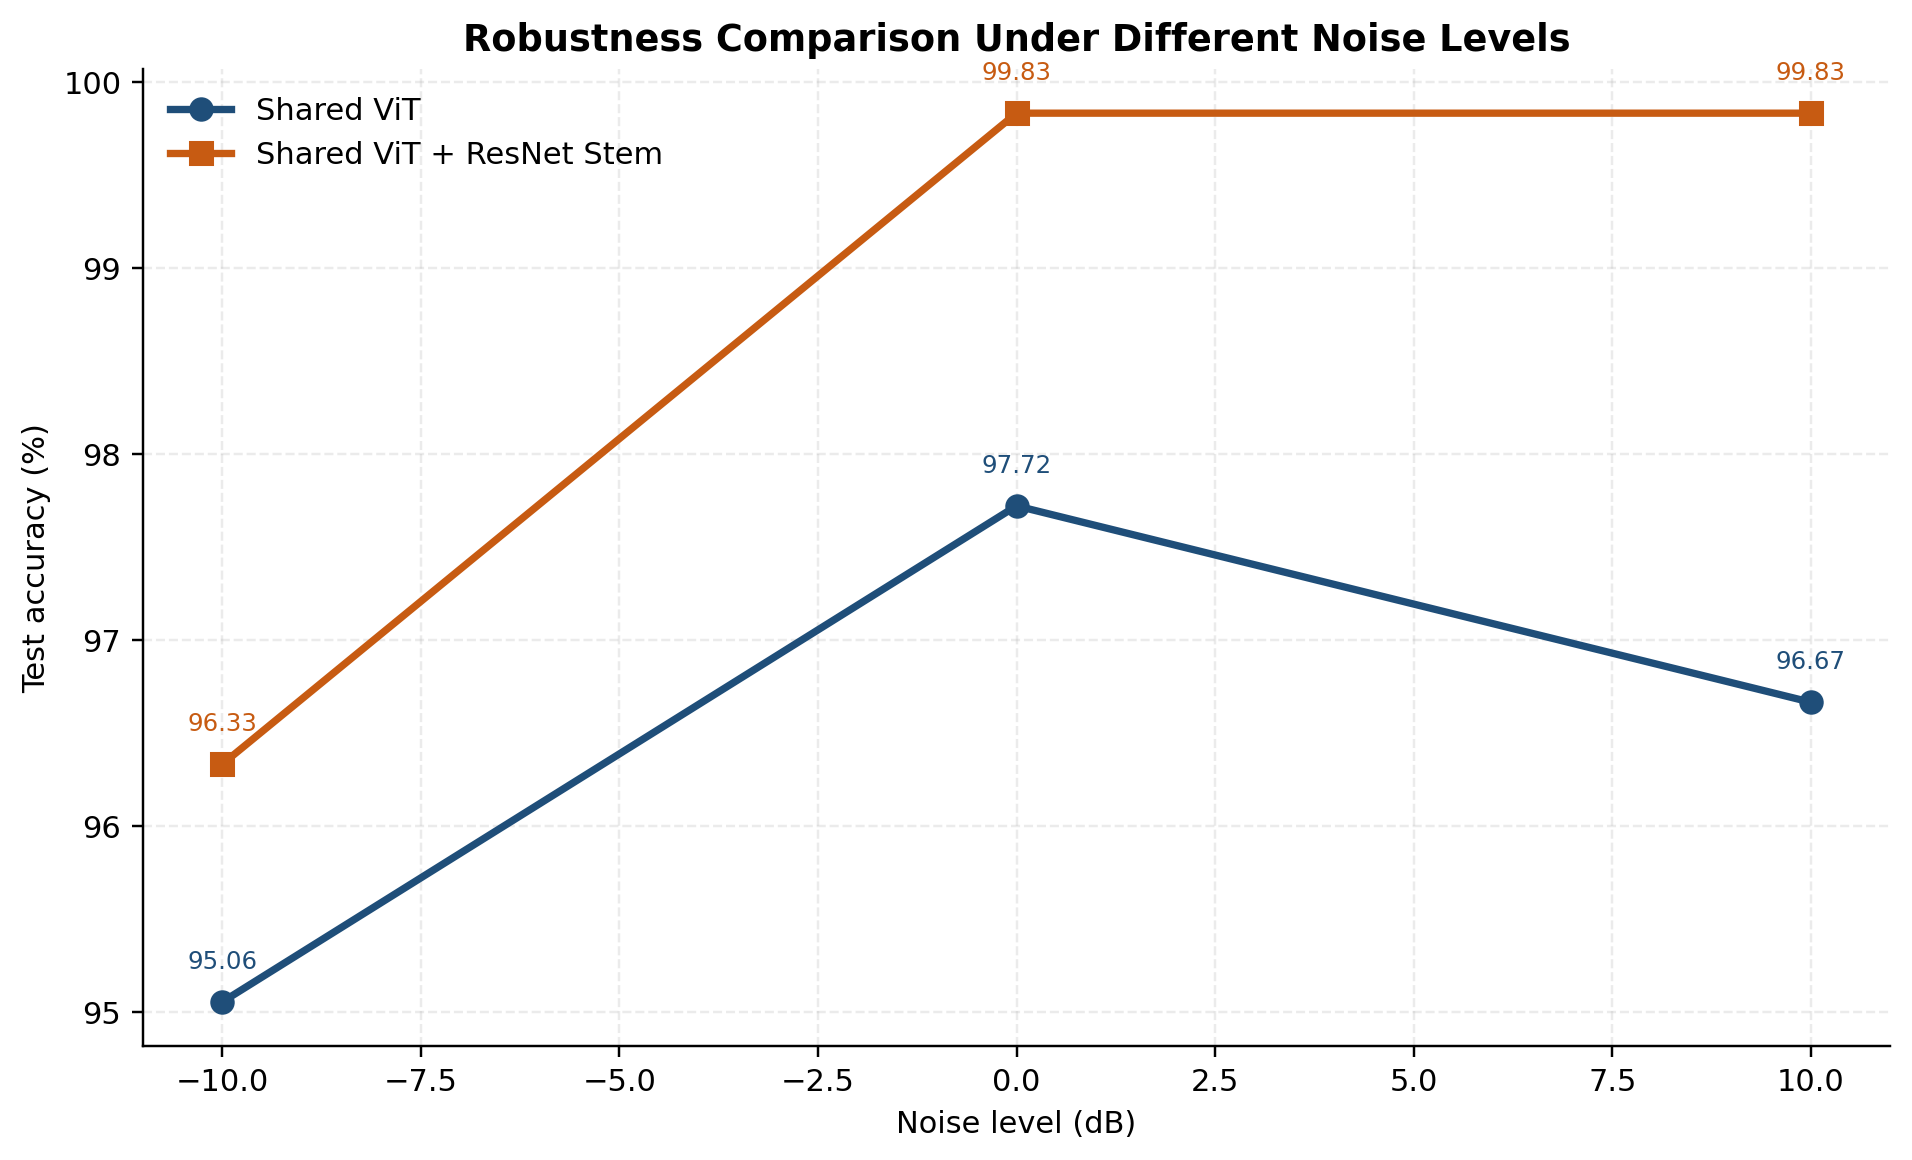
\includegraphics[width=0.82\textwidth]{figures/paper_robustness_main.png}
\caption{Recognition accuracy of the shared-parameter baseline and the proposed RSP-ViT under different Gaussian white noise levels.}
\label{fig:robustness_curve}
\end{figure}

\section{Conclusion}

This paper presented a complete FMCW radar-based human activity recognition framework that integrates 2D FFT-based micro-Doppler generation with a lightweight transformer classifier. A practical preprocessing pipeline was first adopted to convert raw radar echoes into recognition-oriented micro-Doppler images. On this basis, the proposed RSP-ViT combined a ResNet-style convolutional stem with shared-parameter transformer encoding to improve local feature extraction and reduce structural redundancy. Experimental results demonstrated that RSP-ViT achieves a better accuracy-efficiency trade-off than vanilla ViT and MobileNetV2, while also maintaining stable recognition performance under Gaussian white noise. These results verify the effectiveness of the proposed design for compact radar micro-Doppler recognition. Future work will further investigate larger cross-subject datasets, more complex measurement environments, and deployment-oriented optimization for real-time radar perception.

\begin{thebibliography}{11}
\bibitem{Vandersmissen2018}
Vandersmissen, B., Knudde, N., Jalalvand, A., Couckuyt, I., Bourdoux, A., De Neve, W., Dhaene, T.: Indoor person identification using a low-power FMCW radar. IEEE Transactions on Geoscience and Remote Sensing 56(7), 3941--3952 (2018)

\bibitem{Chen2006}
Chen, V.C., Li, F., Ho, S.-S., Wechsler, H.: Micro-Doppler effect in radar: phenomenon, model, and simulation study. IEEE Transactions on Aerospace and Electronic Systems 42(1), 2--21 (2006)

\bibitem{Harmanny2014}
Harmanny, R.I.A., Driessen, H., Janssen, H.W.M.: Radar micro-Doppler feature extraction using the spectrogram and the cepstrogram. In: 11th European Radar Conference (EuRAD), pp. 165--168. IEEE, Rome (2014)

\bibitem{Papanastasiou2021}
Papanastasiou, A., Trommel, R.P., Harmanny, R.I.A., Yarovoy, A.: Deep learning-based identification of human gait by radar micro-Doppler signatures. In: 18th European Radar Conference (EuRAD), pp. 89--92. IEEE, London (2021)

\bibitem{Li2022SemiHAR}
Li, X., He, Y., Jing, X., Zhang, X.: Semisupervised human activity recognition with radar micro-Doppler signatures. IEEE Transactions on Geoscience and Remote Sensing 60, 1--14 (2022)

\bibitem{Du2020SCGRNN}
Du, H., Jin, T., Song, Y., Dai, Y.: Segmented convolutional gated recurrent neural networks for human activity recognition in ultra-wideband radar. Neurocomputing 396, 451--464 (2020)

\bibitem{Huan2023LHViT}
Huan, H., Xu, Y., Zhu, Y., Li, G., Zhang, L.: LH-ViT: A lightweight hybrid vision transformer for radar-based human activity recognition. Scientific Reports 13, 18617 (2023)

\bibitem{He2016ResNet}
He, K., Zhang, X., Ren, S., Sun, J.: Deep residual learning for image recognition. In: Proceedings of the IEEE Conference on Computer Vision and Pattern Recognition (CVPR), pp. 770--778. IEEE, Las Vegas (2016)

\bibitem{Sandler2018MobileNetV2}
Sandler, M., Howard, A., Zhu, M., Zhmoginov, A., Chen, L.-C.: MobileNetV2: Inverted residuals and linear bottlenecks. In: Proceedings of the IEEE/CVF Conference on Computer Vision and Pattern Recognition (CVPR), pp. 4510--4520. IEEE, Salt Lake City (2018)

\bibitem{Dosovitskiy2021ViT}
Dosovitskiy, A., Beyer, L., Kolesnikov, A., Weissenborn, D., Zhai, X., Unterthiner, T., Dehghani, M., Minderer, M., Heigold, G., Gelly, S., Uszkoreit, J., Houlsby, N.: An image is worth 16x16 words: Transformers for image recognition at scale. In: International Conference on Learning Representations (ICLR) (2021)

\bibitem{Lan2020ALBERT}
Lan, Z., Chen, M., Goodman, S., Gimpel, K., Sharma, P., Soricut, R.: ALBERT: A lite BERT for self-supervised learning of language representations. In: International Conference on Learning Representations (ICLR) (2020)
\end{thebibliography}

\end{document}
